Veamos finalmente, en esta pr\'actica, algunas t\'ecnicas de posprocesamiento para im\'agenes satelitales que nos ayudaran a mejorar los valores extraidos y conocer la incerteza en su estimaci\'on. Son nuestros objetivos:

\begin{itemize}
  \item Aplicar filtros modales a las clasificaciones para eliminar p\'ixeles aislados.
  \item Poder calcular la presici\'on total para la clasificaci\'on y sus precisiones del usuario y productor.
  \item Estimar el error de para las areas calculadas a partir de la imagen clasificada.
\end{itemize}

Vamos a usar los paquetes \texttt{raster}, \texttt{rgdal}, \texttt{RStoolbox} y \texttt{rasterVis}.

\section{Filtrado de clasificaciones}

Una de las primeras tareas a realizar luego de clasificar una imagen es aplicar un filtro a la misma que permite eliminar p\'ixeles aislados. Al hacerlo podremos descartar, por ejemplo, pixeles de ciudad en el medio de la selva o de selva en medio de la ciudad. Esta es otra forma de incorporar el contexto espacial a nuestras clasificaciones
\begin{exa}
  Veamos como aplicar un filtro por moda a una imagen clasificada. Comencemos cargando una imagen clasificada en R

  \begin{lstlisting}
      mlc.2016 = raster(raster_data/processed/mlc2016)
  \end{lstlisting}

  Para aplicar el filtro de 3x3 creamos una matriz con unos de 3x3 y usamos
  el comando \texttt{focal} con la funcion \texttt{modal}

  \begin{lstlisting}
    colores = c('#b2df8a','#33a02c',
                '#fdbf6f','#ff7f00',
                '#fb9a99','#e31a1c',
                '#a6cee3','#1f78b4')
    window <- matrix(1,nrow=3, ncol=3)
    mlc.3x3.2016 <-focal(mlc.2016,w=window,fun=modal)
    writeRaster(mlc.3x3.2016,"raster_data/processed/mlc3x3-2016", datatype = "INT1U", overwrite=TRUE)
    plot(mlc.3x3.2016,col=colores)
  \end{lstlisting}
  En el caso de un filtro por moda, estaremos dejando el mayor que mas veces aparezca entre los que rodean al pixel.

  Podemos en este caso mostrar las im\'agenes con y sin el filtro juntas.

  \begin{lstlisting}
    plot(stack(mlc.2016, mlc.3x3.2016),col=colores)
  \end{lstlisting}
  \begin{figure}[h!]
    \centering
    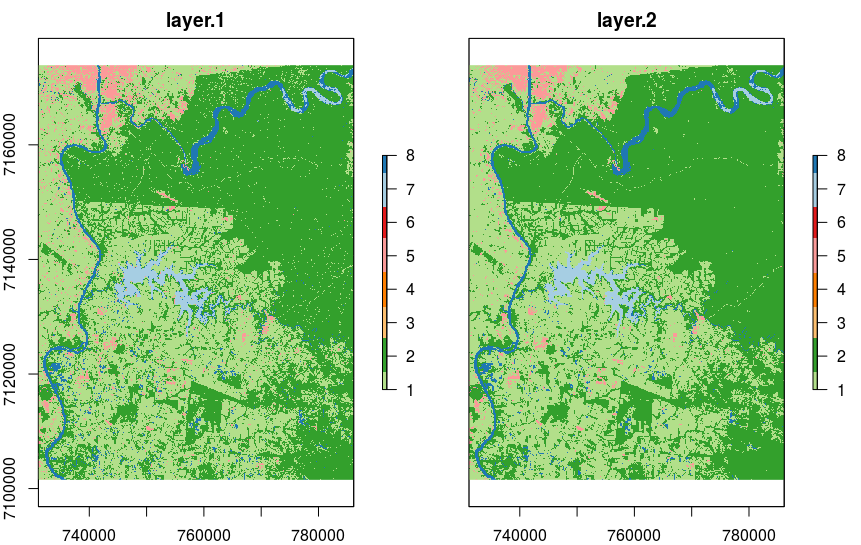
\includegraphics[width=0.7\textwidth]{filtro3x3.png}
    \caption{Imagen de la clasificacion con y sin filtro con una ventana de 3x3.}
    \label{fig:3x3}
  \end{figure}
\end{exa}

\begin{act}
    Aplique filtros de 5x5 y 7x7 para filtrar la imagen. Que problemas desaparecen? que dificultad introducen.
\end{act}

\begin{act}
    Aplique el filtro de 3x3 a la imagen correspondiente al año 2000.
\end{act}

\section{Validacion de clasificaciones}

El segundo procesamiento pos clasificacion, y tal vez el mas importante, es el calculo de la matriz de confusion para nuestra clasificacion. Haremos esto en dos partes: crearemos primero el set de datos para la validacion y luego lo usaremos para calcular dicha matriz.

\begin{exa}
  Veamos como crear un set de puntos aleatorios de muestreo con QGIS. En este caso utilizaremos como unidad de muestreo al pixel, pero de forma similar pueden usarse poligonos o grupos de poligonos.

  Comenzamos abriendo la imagen \file{mlc3x3-2016} en QGIS. Una vez hecho esto, vamos a vectorizar la clasificacion utilizando la herramienta \menu{Raster, Conversion, Poligonizar}. Guardamos el archivo como \file{2016-3x3.shp} en la carpeta de \file{vector\_data} poniendo en nombre del campo \menu{MC\_ID} (figura \ref{fig:poligon}).

  \begin{figure}[h!]
    \centering
    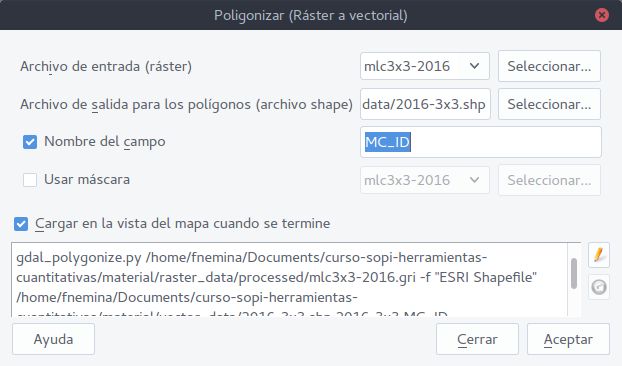
\includegraphics[width=0.7\textwidth]{poligon.png}
    \caption{Menu de poligonizacion}
    \label{fig:poligon}
  \end{figure}

  Una vez hecho esto utilizamos la herramienta \menu{Herramientass de gestion de datos, Dividir capa vectoria} y lo
  guardamos en la carpeta \file{vector\_data,split} (figura \ref{fig:split}).

  \begin{figure}[h!]
    \centering
    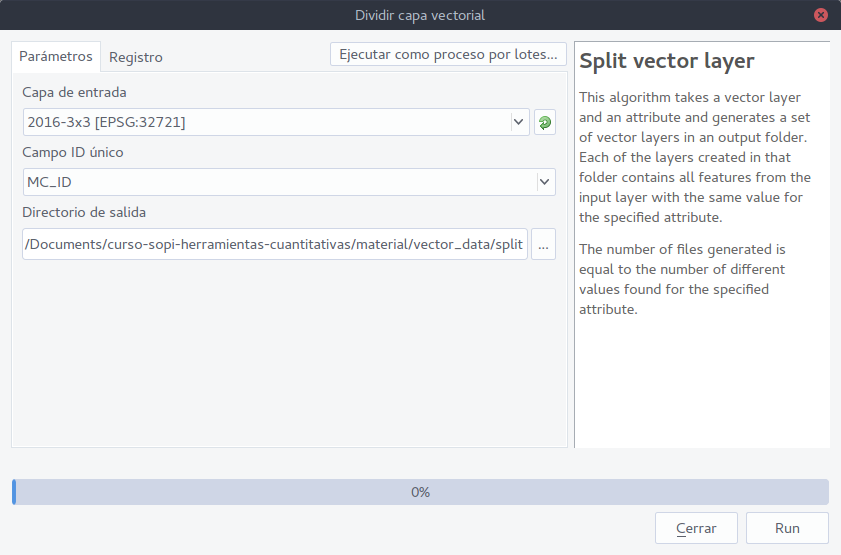
\includegraphics[width=0.7\textwidth]{split.png}
    \caption{Herramienta de division de capa vectorial.}
    \label{fig:split}
  \end{figure}

  Cargamos luego las capas en
  QGIS, elegimos la herramienta \menu{Herramientas de investigacion, Puntos aleatorios en los limites de la capa}
  y hacemos click en el boton \menu{Ejecutar proceso por lotes}. Hacemos click en el boton con los tres puntos y elegimos \menu{Seleccionar del sistema de archivos}.  Seleccionamos cada
  capa y en numero de puntos ponemos la cantidad correspondiente a cada categoria.
  Para calcular dicha cantidad usamos el comando \texttt{freq.2016 <- freq(mlc.3x3.2016)}
  para conocer las frecuencias de aparicion de cada categoria y luego con el comando
  \texttt{freq.2016[,2] <- round(freq.2016[,2]/sum(freq.2016[,2])*250+50)} distribuimos
  los p\'ixeles en cada categoria con 50 fijos y 50 segun la frecuencia de aparicion.
  Con una distancia minima de 100m (figura \ref{fig:dots}).

  \begin{figure}[h!]
    \centering
    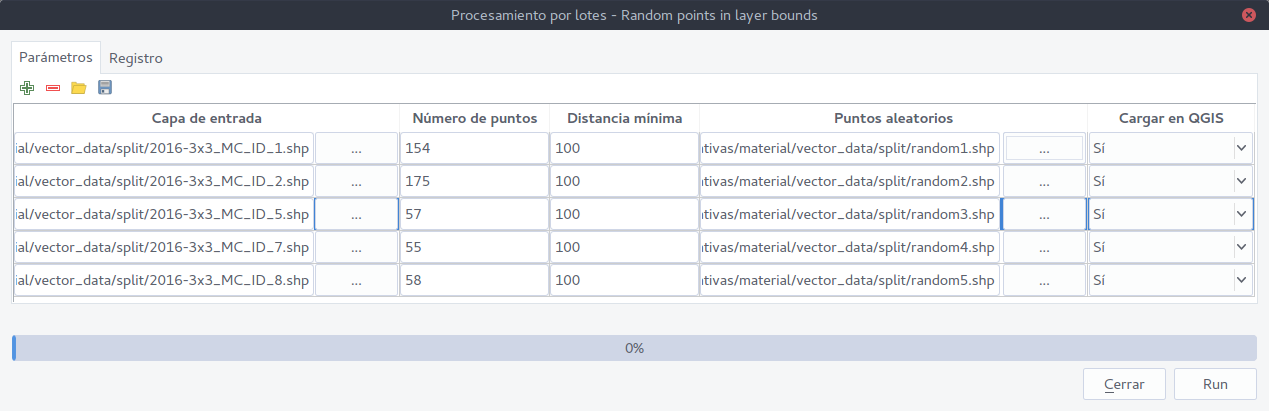
\includegraphics[width=0.7\textwidth]{random-dots.png}
    \caption{Herramienta de creacion de puntos aleatorios.}
    \label{fig:dots}
  \end{figure}

  Elegimos luego en que carpeta guardar los puntos aleatorios y con que nombre y hacemos click en aceptar. Finalmente, una vez creadas las capas de puntos aleatoriosa las unimos utilizando la herramienta \menu{Herramientas de gestion de datos, Combinar capas vectoriales} con el nombre \file{val-2016.shp}.

  \begin{figure}[h!]
    \centering
    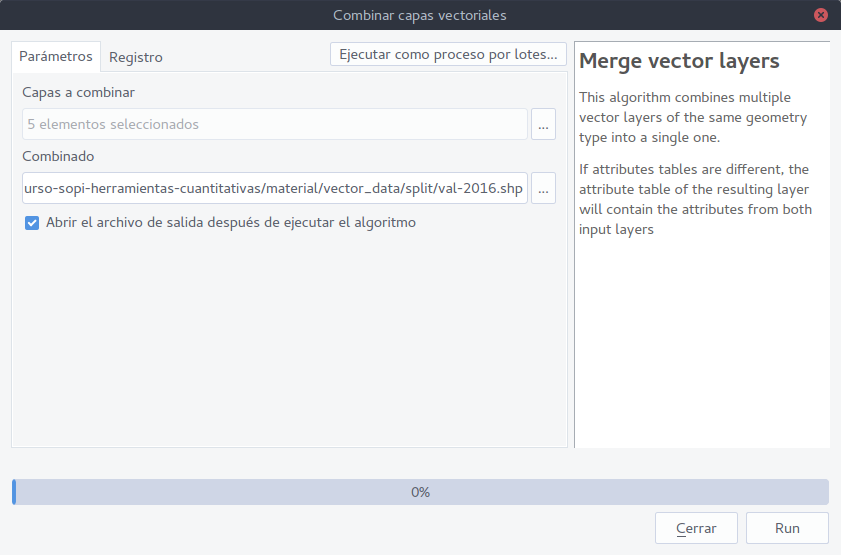
\includegraphics[width=0.7\textwidth]{combinar.png}
    \caption{Combinacion de poligonos en una capa vectorial.}
    \label{}
  \end{figure}

  Una vez unidas las capas editamos la tabla de atributos para agregar el campo
  \verb|MC_ID| y, realizando un analisis visual en distitnas combinaciones de bandas,
  asignamos a cada punto el ID de la clase de informacion a la que pertenece.

  Para hacerlo podemos utilizar la misma imagen que usamos para clasificar o una
  de mayor resolucion espacial. Una vez terminado y guardada la capa tendremos nuestra capa
  de validacion para continuar.

\end{exa}

\begin{act}
  Construya de esta forma una serie de puntos de validacion para la imagen Landsat
  7 del a\~no 2000.
\end{act}

\begin{exa}

  Una vez obtenidos los puntos de validaci\'on podemos calcular la matriz de confusi\'on.
  Para esto debemos cargar el poligono de validacion y la calculamos con la
  funcion \texttt{validateMap}.

  \begin{lstlisting}
      valid.2016 <- readOGR(dsn="vector_data", layer="validacion")
      val.2016 <- validateMap(mlc.3x3.2016,valData = valid.2016,
                                responseCol = "MC_ID")
  \end{lstlisting}

  al inspeccionar el elemento \verb|val.2016$performance| obtenemos la matriz
  de confusion, la presici\'on global como \emph{Acuracy}, la presici\'on del
  productor como \emph{Sensitivity} y la del usuario como \emph{Pos Pred Value}.
  begin

  \begin{Verbatim}[fontsize=\small]
    Confusion Matrix and Statistics

              Reference
    Prediction   1   2   5   7   8
             1 150  27  14   6   2
             2   5 164   0   0   0
             5   6   0  21   0   0
             7   1   0   0  35   5
             8   3   0   0   6  54

    Overall Statistics

                   Accuracy : 0.8497
                     95% CI : (0.8153, 0.8799)
        No Information Rate : 0.3828
        P-Value [Acc > NIR] : < 2.2e-16

                      Kappa : 0.7888
     Mcnemar's Test P-Value : NA

    Statistics by Class:

                         Class: 1 Class: 2 Class: 5 Class: 7 Class: 8
    Sensitivity            0.9091   0.8586  0.60000  0.74468   0.8852
    Specificity            0.8533   0.9838  0.98707  0.98673   0.9795
    Pos Pred Value         0.7538   0.9704  0.77778  0.85366   0.8571
    Neg Pred Value         0.9500   0.9182  0.97034  0.97380   0.9839
    Prevalence             0.3307   0.3828  0.07014  0.09419   0.1222
    Detection Rate         0.3006   0.3287  0.04208  0.07014   0.1082
    Detection Prevalence   0.3988   0.3387  0.05411  0.08216   0.1263
    Balanced Accuracy      0.8812   0.9212  0.79353  0.86570   0.9323
  \end{Verbatim}

  Una vez obtenidas la matriz de confusion y las areas mediante el comando
  \texttt{freq()}, podemos usar el script de R \file{areas.R}. Este nos devolvera
  un archivo csv con la el area del mapa, \emph{adj\_area}, y su error \emph{CI\_adj\_area}
  como se ve al ejecutar el comando \texttt{ov[c(1:5,11,12)]}.
  \begin{Verbatim}[fontsize=\small]
          1     2     5     7     8  adj_area CI_adj_area
    1 0.318 0.053 0.030 0.013 0.004 135500.03   11289.281
    2 0.015 0.488 0.000 0.000 0.000 215369.55    9285.073
    5 0.006 0.001 0.021 0.000 0.000  20265.40    6243.584
    7 0.000 0.000 0.000 0.016 0.003  12318.18    4174.173
    8 0.002 0.000 0.000 0.003 0.028  13907.63    2694.601
  \end{Verbatim}
\end{exa}


\begin{act}
    Construya la matriz de confusion y obtenga la presicion global para todas
    las clasificaciones del a\~no 2000 y 2016. Que algoritmo funciona mejor con la imagen? A partir
    de la misma obtenga estimaciones de area para el a\~no 2000 y 2016 y utilicela
    para estimar la perdida de selva paranaense durante este periodo.
\end{act}
